\section{Theorie}
\label{sec:Theorie}

\subsection{Gedämpfte Schwingungen}
\subsubsection{Schaltkreis}
Der LC-Kreis enthält eine Spule mit Induktivität $L$ und einen Kondensator mit Kapazität $C$ (siehe Abb. \ref{fig:lckreis}).
Die Energie pendelt zwischen den beiden Energiespeichern Spule und Kondensator hin und her.
Hier handelt es sich um einen ungedämpften Oszillator, da die Gesamtenergie im System vollständig erhalten bleibt.
\\\\
In Abbildung \ref{fig:lrckreis} ist der LRC-Kreis abgebildet.
Das System enthält einen Widerstand $R$, Induktivität $L$ und Kapazität $C$.
Die Energie schwingt (wie im LC-Kreis) zwischen Kondensator und Spule hin und her.
Es handelt sich um eine gedämpfte Schwingung, da Energie am Widerstand $R$ in Wärmeenergie umgewandelt wird und die Gesamtenergie im System mit der Zeit abnimmt.

\begin{figure}
    \centering
    \begin{subfigure}{0.48\textwidth}
        \centering
        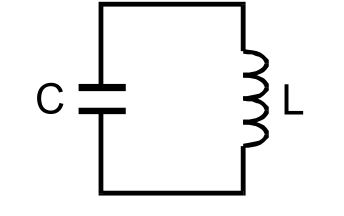
\includegraphics[height=3cm]{content/data/lckreis.jpg}
        \caption{Ungedämpfter Schwingkreis}
        \label{fig:lckreis}
    \end{subfigure}
    \begin{subfigure}{0.48\textwidth}
        \centering
        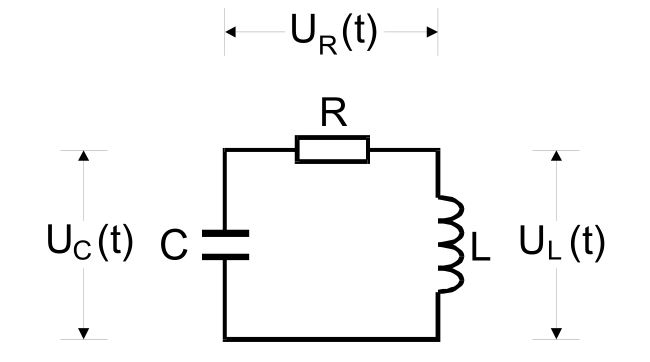
\includegraphics[height=3cm]{content/data/lrckreis.jpg}
        \caption{Gedämpfter Schwingkreis} 
        \label{fig:lrckreis}
    \end{subfigure}
    \caption{Schwingkreise mit den Bauelelementen: Kondensator mit Kapazität $C$, Spule mit Induktivität $L$, ohmscher Widerstand $R$. \cite[S.284]{anleitung}}
\end{figure}

\subsubsection{Differentialgleichung}
Nach dem 2. kirchhoffschen Gesetz, Induktionsgesetz und weiteren Beziehungen für die Spannung $U$, folgt für den LRC-Kreis die Differentialgleichung
\begin{equation}
    \frac{\symup{d}^2I}{\symup{d}t^2} + \frac{R}{L} \frac{\symup{d}I}{\symup{d}t} + \frac{1}{LC} I = 0 .
    \label{eqn:dgl_lrc}
\end{equation}
Der Ansatz
\begin{equation*}
    I(t) = \tilde{I} \mathrm{e}^{i\tilde{\omega} t} \quad \text{mit } \tilde{\omega}, \tilde{I} \in \mathbb{C}
\end{equation*}
löst die Differentialgleichung \autoref{eqn:dgl_lrc}.
Nach einsetzen in die DGL ergibt sich
\begin{equation}
    \tilde{\omega}_{1,2} = i \frac{R}{2L} \pm \sqrt{\frac{1}{LC} - \frac{R^2}{4L^2}} .
    \label{eqn:lrcomega}
\end{equation}
Die allgemeine Lösung
\begin{equation*}
    I(t) = \tilde{I}_1 \mathrm{e}^{i\tilde{\omega}_1 t} + \tilde{I}_2 \mathrm{e}^{i\tilde{\omega}_2 t}
\end{equation*}
ergibt sich durch Linearkombination der einzelnen Lösungen.
Nach einsetzen von $\tilde{\omega}_{1,2}$ \autoref{eqn:lrcomega}, folgt
\begin{equation}
    I(t) = \mathrm{e}^{-2 \pi \mu t} \left ( \tilde{I}_1 \mathrm{e}^{i 2\pi \tilde{\nu} t} + \tilde{I}_2 \mathrm{e}^{-i 2\pi \tilde{\nu} t} \right)
    \label{eqn:dgl_loesung}
\end{equation}
mit den Abkürzungen
\begin{equation}
    2\pi\mu \coloneqq \frac{R}{2L}
    \label{eqn:mu}
\end{equation}
\begin{equation*}
    2\pi\tilde{\nu} \coloneqq \sqrt{\frac{1}{LC} - \frac{R^2}{4L^2}} .
\end{equation*}

\subsubsection{Fallunterscheidung: Lösungsgleichung}
Die Art der gedämpften Schwingung hängt nun von der Form von $\tilde{\nu}$ ab.
Im folgenden werden drei Fälle für $2\pi\tilde{\nu}$ genauer untersucht.\\
\\

%Schwingfall
\textbf{1. Fall: Gedämpfte Schwingung} 
\begin{equation*}
\frac{1}{LC} > \frac{R^2}{4L^2}
\end{equation*}
$\tilde{\nu}$ ist reell. Das bedeutet, die Konstanten müssen $\tilde{I}_1 = \bar{\tilde{I}_1}$ erfüllen.
Nach einigen Umformungen folgt für $I(t)$
\begin{equation}
    I(t) = A_0 \mathrm{e}^{-2\pi\mu t} \cos(2 \pi \nu t + \eta)
\end{equation}
mit  $A_0,\eta \in \mathbb{R}$. Physikalisch beschreibt $\nu$ die Frequenz einer harmonischen Schwingung.
Die Schwingungsdauer
\begin{equation}
    T= \frac{2\pi}{\omega} = \frac{2\pi}{\sqrt{\frac{1}{LC}\frac{R^2}{4L^2}}}
    \label{eqn:schwingfall_T}
\end{equation}
ist konstant. Anders als die Amplitude die mit der Zeit abnimmt.
In einem ungedämpften Schwingkreis ist $R=0$.
Für $R \rightarrow 0$ ergibt sich die Schwingungsdauer (siehe \autoref{eqn:schwingfall_T})
\begin{equation}
    T_0 = 2\pi\sqrt{LC} .
    \label{eqn:T}
\end{equation}
Die Abklinkdauer $T_\text{ex}$ beschreibt den Zeitpunkt, indem die Amplitude um den e-ten Teil ihres Anfangswertes abgenommen hat.
Sie wird nach
\begin{equation}
    T_\text{ex} = \frac{2L}{R}
\end{equation}
berechnet. In Abb. \ref{fig:schwingfall} ist der Verlauf der Stromstärke $I(t)$ zu sehen.
Die abfallende Amplitude der Stromstärke wird durch die Funktion
\begin{equation}
    f(t) = \pm \mathrm{e}^{-2\pi\mu t}
    \label{eqn:einhuellende}
\end{equation}
eingehüllt.

\begin{figure}
    \centering
    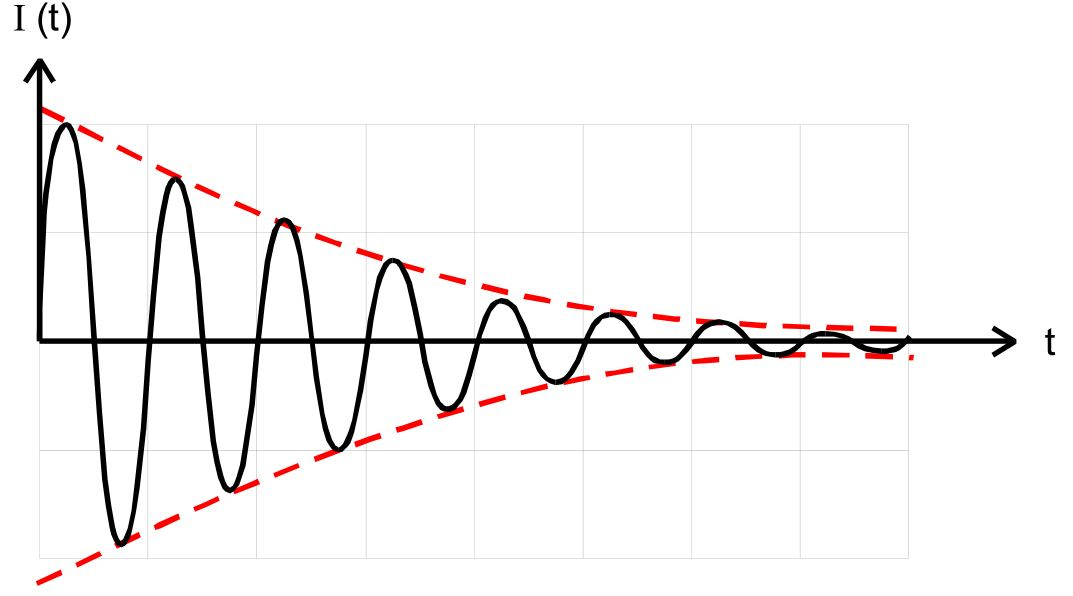
\includegraphics[width=10cm]{content/data/schwingfall.jpg}
    \caption{Schwingfall: Die abfallende Amplitude des Stroms $I(t)$ wird durch \autoref{eqn:einhuellende} beschrieben. \cite[S.287]{anleitung}}
    \label{fig:schwingfall}
\end{figure}

%kriechfall
\textbf{Fall 2: Kriechfall}
\begin{equation*}
    \frac{1}{LC} < \frac{R^2}{4L^2}
\end{equation*}
Hier ist $\tilde{\nu}$ imaginär und daher $I(t)$ (siehe \autoref{eqn:dgl_loesung}) reell.
Der Stromverlauf beschreibt keine Schwingung mehr, sondern ein einfaches Relaxationsverhalten.
In Abb. \ref{fig:aperiodisch} zeigen die durchgezogenen Linien verschiedene Lösungen des Kriechfalls.
Nach hinreichender Zeit gilt für die Stromstärke $I(t)$ 
\begin{equation}
    I(t) \propto \mathrm{e}^{-\left( \frac{R}{2L} - \sqrt{\frac{R^2}{4L^2}-\frac{1}{LC}} t \right)} .
\end{equation}

%aperiodischer Grenzfall
\textbf{3. Fall: aperiodischer Grenzfall}
\begin{equation}
    \frac{1}{LC} = \frac{R_\text{ap}^2}{4L^2}
    \label{eqn:aperiodisch}
\end{equation}
Hier ist $\nu = 0$ und für die Stromstärke $I(t)$ folgt
\begin{equation}
    I(t) = A \mathrm{e}^{-\frac{R}{2L}t} = A \mathrm{e}^{-\frac{1}{\sqrt{LC}}} .
\end{equation}
Es ist kein Nulldurchgang bzw. Überschwingung möglich.
$I(t)$ verläuft am schnellsten aller Lösungen gegen 0.
Die gestrichelte Linie in Abb. \ref{fig:aperiodisch} zeigt den Verlauf des aperiodischen Grenzfall.
\begin{figure}
    \centering
    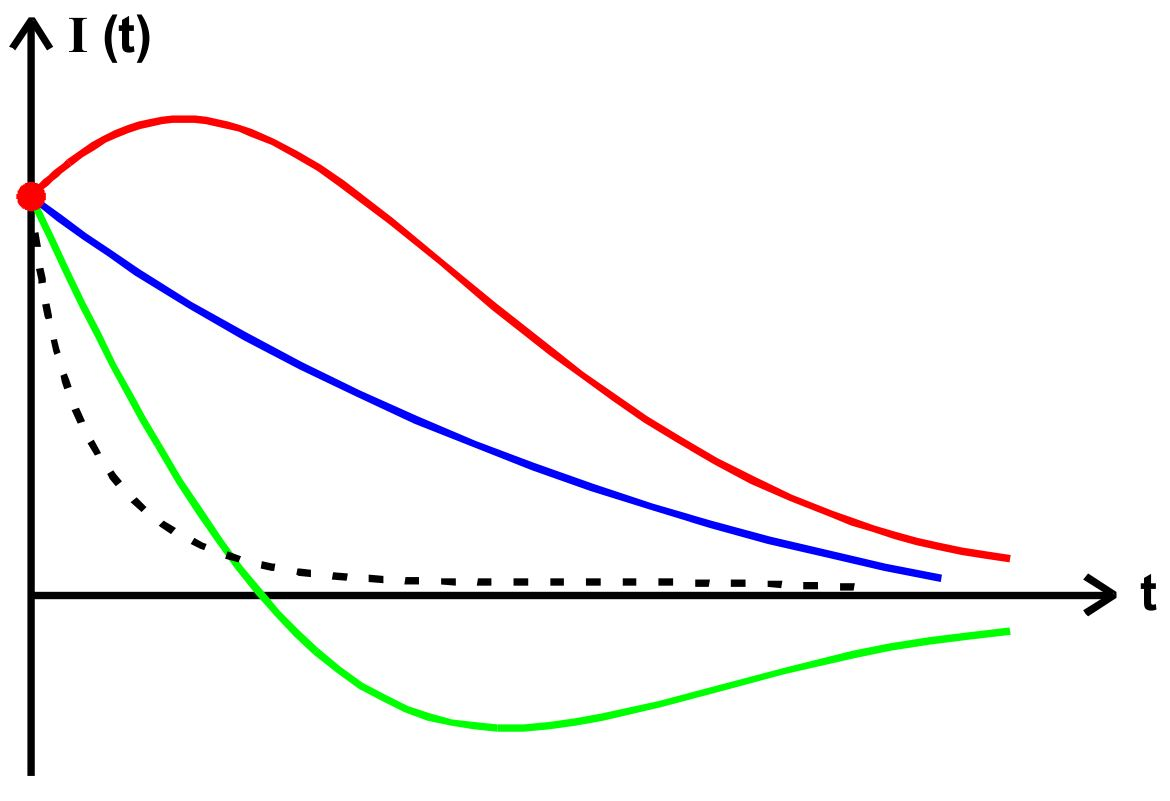
\includegraphics[width=10cm]{content/data/aperiodisch.jpg}
    \caption{Verschiedene Verläufe des Kriechfalls und der aperiodische Grenzfall (gestrichelte Kurve) dargestellt. \cite[S.288]{anleitung}}
    \label{fig:aperiodisch}
\end{figure}
\FloatBarrier
\subsection{Erzwungene Schwingung}
\subsubsection{Schaltkreis}
In den gedämpften Schwingkreis wird zusätzlich eine Spannungsquelle verbaut und eine Sinusspannung eingeschaltet.
In Abb. \ref{fig:erzw_schwingkreis} ist ein Schaltplan einer erzwungenen Schwingung.
Die Wechselspannung hat die Form
\begin{equation}
    U(t) = U_0 \mathrm{e}^{i\omega t} .
\end{equation}
\begin{figure}
    \centering
    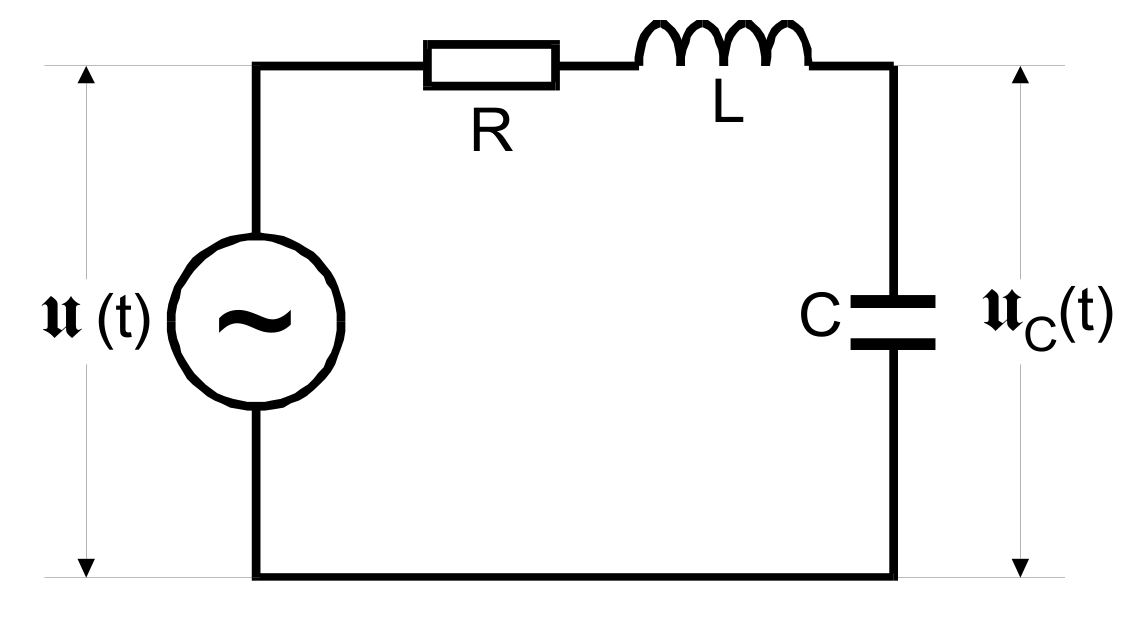
\includegraphics[width=8cm]{content/data/erzw_schwingkreis.jpg}
    \caption{Schaltplan einer erzwungenen Schwingung mit Erregerfrequenz $U(t)$. \cite[S.289]{anleitung}}
    \label{fig:erzw_schwingkreis}
\end{figure}

\subsubsection{Differential- und Lösungsgleichungen}
Die Differentialgleichung
\begin{equation}
    LC \frac{\symup{d}^2U_\text{c}}{\symup{d}t^2} + RC \frac{\symup{d}U_\text{c}}{\symup{d}t + U_\text{c}} = U_0 \mathrm{e}^{i\omega t}
    \label{eqn:dgl_erzwungen}
\end{equation}
lässt sich mit dem Ansatz
\begin{equation*}
    U_\text{c}(\omega,t) = U(\omega) \mathrm{e}^{i\omega t}
\end{equation*}
lösen. Nach einsetzen in die DGL (\autoref{eqn:dgl_erzwungen}) und auflösen nach $U$ ergibt sich
\begin{equation}
    U = \frac{U_0}{1 - LC \omega^2 + i\omega RC} = \frac{U_0 (1-LC \omega^2 - i\omega RC)}{(1-LC\omega^2)^2 + \omega^2 R^2 C^2}
\end{equation}
für die Spannung.
Die Phase
\begin{equation}
    \varphi(\omega) = \arctan \left( \frac{-\omega RC}{1-LC\omega^2} \right)
\end{equation}
folgt aus $\tan \varphi(\omega) = \frac{Im(U)}{Re(U)}$.
Die Spannung am Kondensator kann mit
\begin{equation}
    U_\text{c}(\omega) = \frac{U_0}{\sqrt{\left( 1 - LC\omega^2 \right)^2 + \omega^2R^2C^2}}
    \label{eqn:spannung_c}
\end{equation}
ermittelt werden. Für $U_\text{c}$ gilt $U_\text{c}(\omega)\xrightarrow{\omega\to\infty}0$ und $U_\text{c}(\omega)\xrightarrow{\omega\to 0}U_0$.
Die Spannung besitzt ein Maximalwert bei der Frequenz
\begin{equation}
    \omega_\text{res} = \sqrt{\frac{1}{LC} - \frac{R^2}{2L^2}} .
\end{equation}
Die Frequenz wird als Resonanzfrequenz bezeichnet.\\
Wenn
\begin{equation*}
    \frac{R^2}{2L^2} << \frac{1}{LC}
\end{equation*}
gilt, wird von schwacher Dämpfung gesprochen und $\omega_\text{res}$ nähert sich $\omega_0$ der ungedämpften Schwingung an.
Also folgt für $U_\text{c}$
\begin{equation}
    U_\text{c,max} = \frac{1}{\omega_0 RC} U_0 = \frac{1}{R} \sqrt{\frac{L}{C}}U_0 .
\end{equation}
Wenn nun $R \rightarrow 0$ geht, so folgt die Resonanzkatastrophe $U_\text{c,max} \rightarrow \infty$.
Die Resonanz kann durch die Breite der Kurve (\autoref{eqn:spannung_c}) quantifiziert werden.
Die Frequenzen $\omega_+$ und $\omega_-$ geben an, wo $U_\text{c}$ um den Faktor $1/\sqrt{2}$ vom Maximalwert gesunken ist.
Sie können nach
\begin{equation}
    \omega_+ - \omega_- \thickapprox \frac{R}{L}
    \label{eqn:guete1}
\end{equation}
ermittelt werden. Als Maß des Resonanz kann 
\begin{equation}
    q = \frac{\omega_0}{\omega_+ - \omega_-} = \frac{1}{\omega_0RC} \quad \text{mit } \omega_0 = \frac{1}{\sqrt{LC}}
\end{equation}
verwendet werden. Es gibt den Faktor, um den die maximale Kondensatorspannung $U_\text{c,max}$ gegenüber der Erregerspannung erhöht ist an.
\\
Eine starke Dämpfung liegt vor, wenn
\begin{equation*}
    \frac{R^2}{2L^2} >> \frac{1}{LC}
\end{equation*}
gilt. Hier existiert keine Resonanzerhöhung, sondern $U_\text{c}$ geht vom Anfangswert $U_0$ gegen 0.
Ist die Phase gerade $\pi/2$ oder $\frac{3}{4}\pi$, so gilt
\begin{equation}
    \omega_{1,2} = \pm \frac{R}{2L} + \sqrt{\frac{R^2}{4L^2} + \frac{1}{LC}} 
\end{equation}
und es ergibt sich
\begin{equation}
    \omega_1 - \omega_2 = \frac{R}{L} ,
    \label{eqn:breite}
\end{equation}
genauso wie bei der schwachen Dämpfung (\autoref{eqn:guete1}).